\qns{[OPTIONAL] DFT Secret Code}

Your friend sends you a secret message in the form of a voltage signal, with a cipher that depends on the DFT of the signal. You decide to sample the signal at 2 Hz and get the following data:
\newline
\begin{center}
    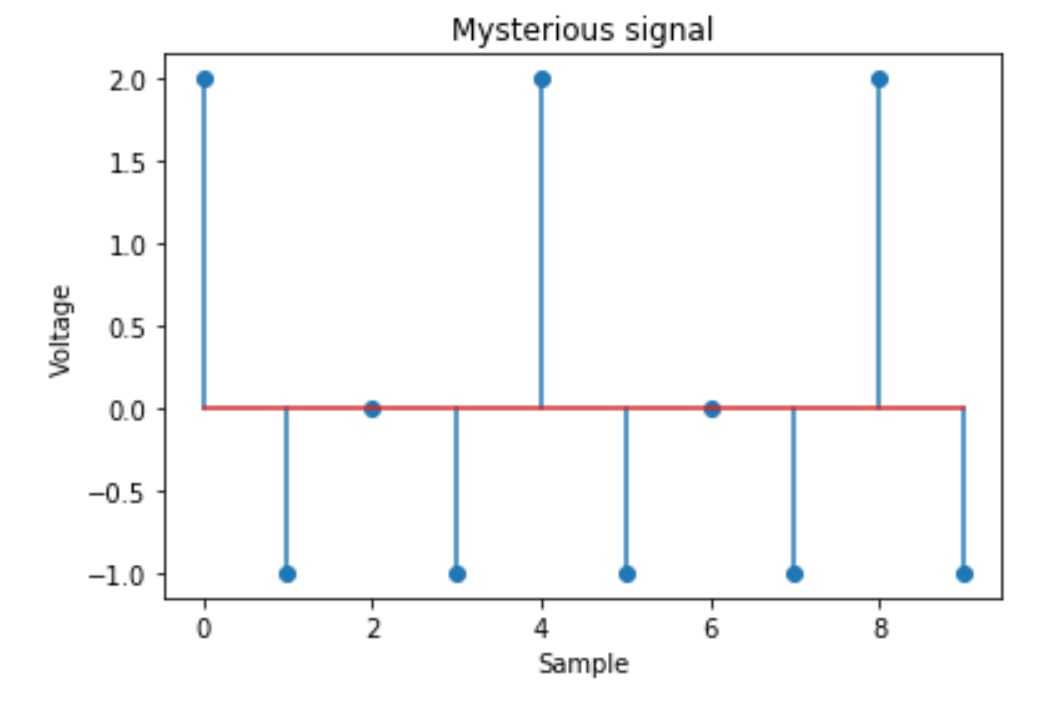
\includegraphics[width = 0.5 \textwidth]{\bank/dft/figures/mysterious_signal.PNG} 
\end{center}

\begin{enumerate}
    \qitem What is the period of this signal (in samples and seconds)? Following from that, what is the fundamental frequency (in radians per second) and what dimension of DFT should we perform?

    \sol{
        The signal repeats every 4 samples, so the period is \textbf{4 samples} and we should take a \textbf{4-dimensional DFT}. We are taking two samples a second, so the period is \textbf{2 seconds}. The fundamental frequency is $2\pi/\text{period} = \pi$.
    }

    \qitem You want to ascertain what you can about the signal without taking the DFT directly. Your friend gave you the hint that it is the sum of cosines with amplitude 1. Find $f(t)$, a function that represents your signal with respect to time. Assume no aliasing.

    \sol {
        List out information you have about the signal:
        \begin{itemize}
            \item The fundamental frequency is $\pi$, so the cosines have frequencies that are integer multiples of $\pi$. 
            \item We are assuming no aliasing, so there are no frequencies above $2\pi \cdot \text{sampling frequency} / 2$, or $2\pi$. 
            \item So, the only possible frequencies in our signal are $\pi$ and $2\pi$. 
            \item The signal is not a simple cosine, so it must have both frequencies.
            \item Both cosines have amplitude 1, and the signal has amplitude 2 at the first sample, so neither have a phase shift.
        \end{itemize}
        So,
        $$f(t) = \cos(\pi t) + \cos(2\pi t)$$
    }

    \qitem What is the $\vec{X}$, the N-dimensional DFT of the signal, where N is the dimension we found in part (a)?

    \sol {
        First, write out our signal in terms of the sample number. We're sampling twice a second, so 
        $$x(n) = \cos(\pi(n/2)) + \cos(2\pi (n/2)) = \cos(\pi/2 n) + \cos(\pi n)$$ 
        Writing $x(n)$ as a sum of complex exponentials, we have
        \begin{align*}
            x(n) = e^{j(\pi/2)n} + e^{-j(\pi/2)n} + e^{j\pi n} + e^{-j\pi n} \\
            = e^{j(\pi/2)n} + e^{j(3\pi/2)n} + 2e^{j\pi n}
        \end{align*}
        Representing the $k^{\text{th}}$ DFT basis vector as $\vec{\phi}_k(n) = e^{jk(\pi/2)n}$, we can rewrite $\vec{x}$ as
        $$\vec{x} = \vec{\phi}_1 + 2\vec{\phi}_2 + \vec{\phi}_3$$
        So,
        $$\vec{X} = \begin{bmatrix} 0 & 1 & 2 & 1 \end{bmatrix}^T$$
    }

    \qitem When you try to decode the message, you get nonsense! Why could this be the case? \\
    \textit{Hint: what assumption did we make in taking the DFT of this signal?}

    \sol {
        Remember that in part (b) we assumed that there was no \textbf{aliasing}. However, we can only make that assumption if we know that we are sampling at at least twice the highest frequency of the signal. If there are higher-frequency signals present, they will show up as lower frequencies when we sample and run the DFT.
    }

    \qitem You talk to your friend and find out that all angular frequencies in the signal are between $0$ and $5\pi$. Given that information, what is the function, $f(t)$, that represents your signal?

    \sol {
        To see what frequencies could be in the signal, let's look at $x(n)$.
        $$x(n) = \cos(\pi/2 n) + \cos(\pi n)$$
        In discrete time, cosine waves are $2\pi$ periodic in frequency, so
        $$\cos(\omega n) = \cos((\omega + 2\pi)n)$$
        Then, our signal in discrete time could have the frequencies $\pi/2 + 2k\pi$ and $\pi + 2l\pi$, where $k$ and $l$ are integers:
        $$x(n) = \cos((\pi/2 + 2k\pi) n) + \cos((\pi + 2l\pi) n)$$
        Converting to continuous time, we have
        $$f(t) = \cos((\pi + 4k\pi)t) + \cos((2\pi + 4l\pi)t)$$
        Given that all frequencies must be between $0$ and $5\pi$, our signal must be:
        $$f(t) = \cos(2\pi t) + \cos(5\pi t)$$
        \textit{Note: $f(t) = \cos(2\pi t) + \cos(3\pi t)$ is also a valid answer. You can get that answer by setting $k = -1$, which would give us $f(t) = \cos(2\pi t) + \cos(-3\pi t)$. Cosine is an even function, so $\cos(-3\pi t) = \cos(3\pi t)$}
    }

    \qitem To avoid aliasing, what frequency should you have sampled the signal at? What dimension of DFT should you have used?

    \sol {
        The highest angular frequency is $5\pi$, so the highest linear frequency is $5/2$. We need to sample at twice that rate to avoid aliasing, so we should have had a sampling frequency of at least \textbf{5 Hz}. If we write the signal in terms of samples, we have
        $$x(n) = \cos(2\pi (n/5)) + \cos(5\pi(n/5)) = \cos(2\pi/5 n) + \cos(\pi n)$$
        This signal has a period of 10 samples, so we should use a \textbf{10-dimensional DFT}.
    }

    \qitem What is the DFT of the actual signal?

    \sol {
        In discrete time, our signal is
        $$x(n) = \cos(2\pi/5 n) + \cos(\pi n)$$
        Converting to complex exponentials, we have
        \begin{align*}
             x(n) = e^{j(2\pi/5)n} + e^{-j(2\pi/5)n} + e^{j\pi n} + e^{-j\pi n} \\
            = e^{j(2\pi/5)n} + e^{j(8\pi/5)n} + 2e^{j\pi n}
        \end{align*}
        Representing the $k^{\text{th}}$ DFT basis vector as $\vec{\phi}_k(n) = e^{jk(\pi/5)n}$, we can rewrite $\vec{x}$ as
        $$\vec{x} = \vec{\phi}_2 + 2\vec{\phi}_5 + \vec{\phi}_8$$
        So,
        $$\vec{X} = \begin{bmatrix} 0 & 0 & 1 & 0 & 0 & 2 & 0 & 0 & 1 & 0 \end{bmatrix}^T$$
    }

\end{enumerate}